\documentclass{beamer}
\usepackage[latin1]{inputenc}
\usepackage{xcolor}
\usepackage{hyperref}
\usepackage{minted}
\usepackage{graphicx}
\usepackage{tikz}
\usetikzlibrary{fadings}

\usetheme{default}
\usecolortheme{default}

\title{COMP3320 Introduction to OpenGL}
\author{Alex Biddulph}
\institute{
    The University of Newcastle, Australia
    \and
    Based on the work provided at \url{www.learnopengl.com}
}
\date{Semester 2, 2019}

\begin{document}

\begin{frame}
\titlepage
\end{frame}

\begin{frame}[fragile]{Vertex Attributes}
    \begin{itemize}
        \item Allows us to specify auxilliary data for each vertex
        \item Colour, texture coordinates, etc.
        \item An example specifying vertex colour information
\begin{minted}{c++}
    float vertices[] = {
        // positions         // colors
         0.5f, -0.5f, 0.0f,  1.0f, 0.0f, 0.0f,
        -0.5f, -0.5f, 0.0f,  0.0f, 1.0f, 0.0f,
         0.0f,  0.5f, 0.0f,  0.0f, 0.0f, 1.0f };
\end{minted}
        \item Must specify offset and stride for {\color{blue}\verb"glVertexAttribPointer"}
        \item[] 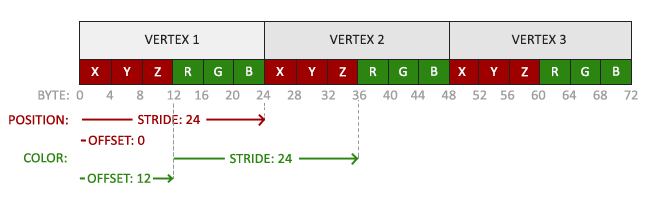
\includegraphics[width=0.90\textwidth]{images/vertex_attribute_pointer_interleaved.png}
    \end{itemize}
    \vfill{}
    {\footnotesize{Image sourced from \url{learnopengl.com/Getting-started/Shaders}}}
\end{frame}

\begin{frame}[fragile]{Vertex Attributes}
    Result should look like this
    \begin{center}
        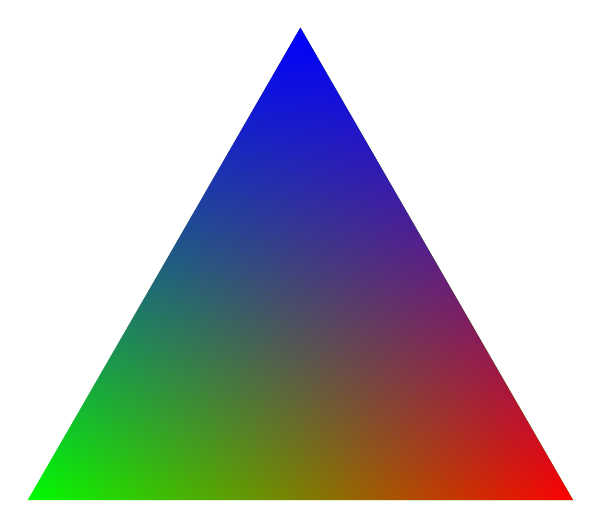
\begin{tikzpicture}
            \fill[green] (90:4) -- (210:4) -- (-30:4) -- cycle;
            \fill[red,path fading=west] (90:4) -- (210:4) -- (-30:4) -- cycle;
            \fill[blue,path fading=south] (90:4) -- (210:4) -- (-30:4) -- cycle;
        \end{tikzpicture}
    \end{center}
\end{frame}

\begin{frame}[fragile]{Textures}
    \begin{itemize}
        \item Rather than using colours to add detail to an object, use an image
        \item Easier to add a lot of detail to an object
        \item To apply a texture we just need to assign texture coordinates to each vertex
\footnotesize{
\begin{minted}{c++}
float vertices[] = {
    // positions         // colors         // textures
     0.5f, -0.5f, 0.0f,  1.0f, 0.0f, 0.0f, 1.0f, 0.0f, 
    -0.5f, -0.5f, 0.0f,  0.0f, 1.0f, 0.0f, 0.0f, 0.0f, 
     0.0f,  0.5f, 0.0f,  0.0f, 0.0f, 1.0f, 0.5f, 1.0f };
\end{minted}
}
        \item[] 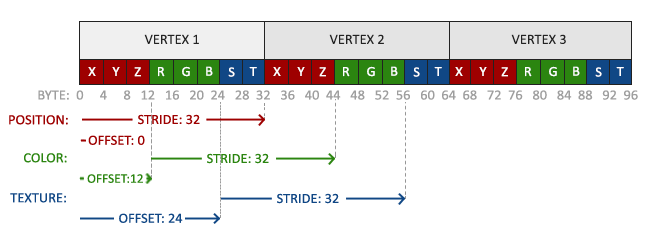
\includegraphics[width=0.90\textwidth]{images/vertex_attribute_pointer_interleaved_textures.png}
    \end{itemize}
    \vfill{}
    {\footnotesize{Image sourced from \url{learnopengl.com/Getting-started/Textures}}}
\end{frame}

\begin{frame}[fragile]{Texture Wrapping}
    \begin{itemize}
        \item Texture coordinates range from $\left(0, 0\right) \to \left(1, 1\right)$
        \item What should happen if coordinates outside this range are specified?
        \item[] 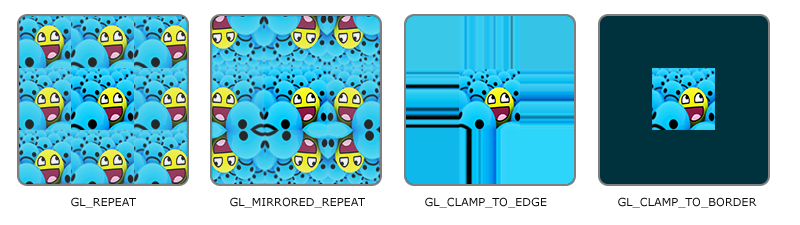
\includegraphics[width=0.90\textwidth]{images/texture_wrapping.png}
        \item Specify behaviour using {\color{blue}\verb"glTexParameteri"}
        \item Specify border colour using {\color{blue}\verb"glTexParameterfv"}
    \end{itemize}
    \vfill{}
    {\footnotesize{Image sourced from \url{learnopengl.com/Getting-started/Textures}}}
\end{frame}

\begin{frame}[fragile]{Texture Filtering}
    \begin{itemize}
        \item Floating-point texture coordinates are mapped to integer pixel coordinates
        \item What should happen if texture coordinates have a fractional component?
        \begin{itemize}
            \item For example, texture coordinates $\left(0.75, 0.0\right)$ maps to pixel coordinates 
                $\left(480.3, 300\right)$
        \end{itemize}
        \item[] \begin{center}
\includegraphics[width=0.40\textheight]{images/texture_filtering.png}\end{center}
        \item Specify behaviour using {\color{blue}\verb"glTexParameteri"}
        \item Behaviour can be specified for both minifying and magnifying operations
    \end{itemize}
    \vfill{}
    {\footnotesize{Image sourced from \url{learnopengl.com/Getting-started/Textures}}}
\end{frame}

\begin{frame}[fragile]{MipMaps}
    \begin{itemize}
        \item No need to use a high resolution image to texture an object a long distance away
        \item Can also result in undesirable artifacts on small objects
        \item The solution?
        \begin{itemize}
            \item Create multiple scaled down versions of the high resolution image
            \item Select a different scaled down texture based on the distance from the camera
        \end{itemize}
        \item[] \begin{center}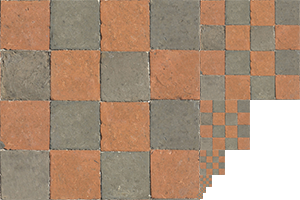
\includegraphics[width=0.40\textheight]{images/mipmaps.png}\end{center}
        \item Generating mipmaps is cumbersome, use {\color{blue}\verb"glGenerateMipmaps"}
        \item Can change mipmap filtering behaviour for minifying and magnifying operations as well
    \end{itemize}
    \vfill{}
    {\footnotesize{Image sourced from \url{learnopengl.com/Getting-started/Textures}}}
\end{frame}

\begin{frame}[fragile]{Loading Textures}
    \begin{itemize}
        \item A number of C/C++ libraries available for loading images 
        \item SOIL is a common library specifically targetting OpenGL
        \item Use {\color{blue}\verb"glGenTexture"} to generate a texture object
        \item Use {\color{blue}\verb"glBindTexture"} to bind a texture object and make it active, be sure to do this 
            before rendering objects
        \item Use {\color{blue}\verb"glTexImage2D"} to attach the raw texture data to the texture object
        \item Generate mipmaps after attaching the raw texture data
        \item It is now safe to delete any pointers to the raw texture data
        \item It is possible to use multiple textures in a single program, use {\color{blue}\verb"glActiveTexture"} to 
            select which texture unit to use before binding
        \begin{itemize}
            \item Should be a minimum of $16$ texture units available
        \end{itemize}
    \end{itemize}
\end{frame}

\begin{frame}[fragile]{Textures}
    Result should look like this

    \begin{center}
        \begin{tikzpicture}[baseline={([yshift=-1em] current bounding box.north)}]
            % Grid lines
            \draw[step=0.5,lightgray,thin] (-1.5, -1.5) grid (1.5, 1.5);

            % Window edges
            \draw[thick] (-1.5, -1.5) -- (-1.5, 1.5) -- (1.5, 1.5) -- (1.5, -1.5) -- cycle;

            % Triangle
            \def\triangle{(-1.5, -1.5) -- (0.0, 1.5) -- (1.5, -1.5) -- cycle}
            \begin{scope}
                \clip \triangle;
                \node {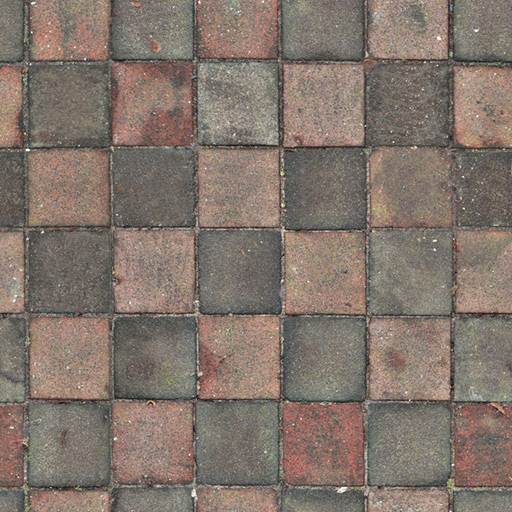
\includegraphics[width=0.3\linewidth]{images/wall.jpg}};
            \end{scope}
            \draw[black, thick] \triangle;

            % Coordinates
            \draw (-1.5, -1.5) node[below left]{$\left(0, 0\right)$};
            \draw ( 1.5,  1.5) node[above right]{$\left(1, 1\right)$};
            \draw (-1.5,  1.5) node[above left]{$\left(0, 1\right)$};
            \draw ( 1.5, -1.5) node[below right]{$\left(1, 0\right)$};
        \end{tikzpicture}
    \end{center}
    \vfill{}
    {\footnotesize{Brick wall image sourced from \url{learnopengl.com/Getting-started/Textures}}}
\end{frame}

\end{document}
